\documentclass[tikz]{standalone}
\usetikzlibrary{shapes}
\begin{document}
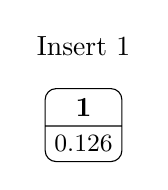
\begin{tikzpicture}[sibling distance=10em,every node/.style = {draw, align=center, shape=rectangle split,rectangle split parts=2, rounded corners}]
\node(root) { \textbf{1}\nodepart{second}{\small 0.126}} ;
\node[shape=rectangle,draw=none,above of=root] {Insert 1};
\end{tikzpicture}
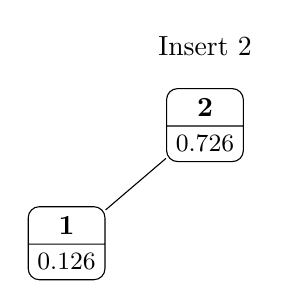
\begin{tikzpicture}[sibling distance=10em,every node/.style = {draw, align=center, shape=rectangle split,rectangle split parts=2, rounded corners}]
\node(root) { \textbf{2}\nodepart{second}{\small 0.726}} 
child[xshift=-5em] { node { \textbf{1}\nodepart{second}{\small 0.126}}  };
\node[shape=rectangle,draw=none,above of=root] {Insert 2};
\end{tikzpicture}
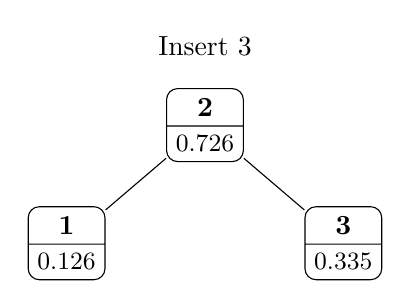
\begin{tikzpicture}[sibling distance=10em,every node/.style = {draw, align=center, shape=rectangle split,rectangle split parts=2, rounded corners}]
\node(root) { \textbf{2}\nodepart{second}{\small 0.726}} 
child { node { \textbf{1}\nodepart{second}{\small 0.126}}  }
child { node { \textbf{3}\nodepart{second}{\small 0.335}}  };
\node[shape=rectangle,draw=none,above of=root] {Insert 3};
\end{tikzpicture}
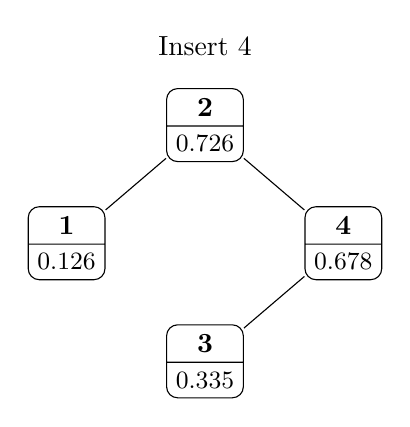
\begin{tikzpicture}[sibling distance=10em,every node/.style = {draw, align=center, shape=rectangle split,rectangle split parts=2, rounded corners}]
\node(root) { \textbf{2}\nodepart{second}{\small 0.726}} 
child { node { \textbf{1}\nodepart{second}{\small 0.126}}  }
child { node { \textbf{4}\nodepart{second}{\small 0.678}} 
child[xshift=-5em] { node { \textbf{3}\nodepart{second}{\small 0.335}}  } };
\node[shape=rectangle,draw=none,above of=root] {Insert 4};
\end{tikzpicture}
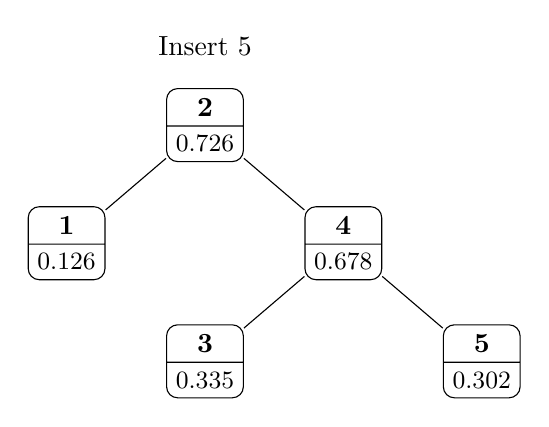
\begin{tikzpicture}[sibling distance=10em,every node/.style = {draw, align=center, shape=rectangle split,rectangle split parts=2, rounded corners}]
\node(root) { \textbf{2}\nodepart{second}{\small 0.726}} 
child { node { \textbf{1}\nodepart{second}{\small 0.126}}  }
child { node { \textbf{4}\nodepart{second}{\small 0.678}} 
child { node { \textbf{3}\nodepart{second}{\small 0.335}}  }
child { node { \textbf{5}\nodepart{second}{\small 0.302}}  } };
\node[shape=rectangle,draw=none,above of=root] {Insert 5};
\end{tikzpicture}
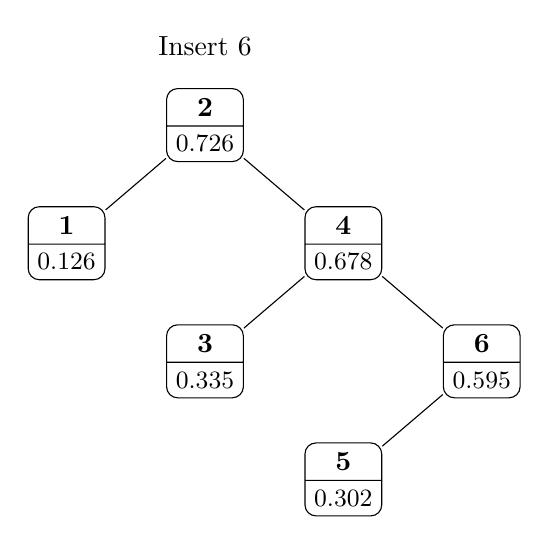
\begin{tikzpicture}[sibling distance=10em,every node/.style = {draw, align=center, shape=rectangle split,rectangle split parts=2, rounded corners}]
\node(root) { \textbf{2}\nodepart{second}{\small 0.726}} 
child { node { \textbf{1}\nodepart{second}{\small 0.126}}  }
child { node { \textbf{4}\nodepart{second}{\small 0.678}} 
child { node { \textbf{3}\nodepart{second}{\small 0.335}}  }
child { node { \textbf{6}\nodepart{second}{\small 0.595}} 
child[xshift=-5em] { node { \textbf{5}\nodepart{second}{\small 0.302}}  } } };
\node[shape=rectangle,draw=none,above of=root] {Insert 6};
\end{tikzpicture}
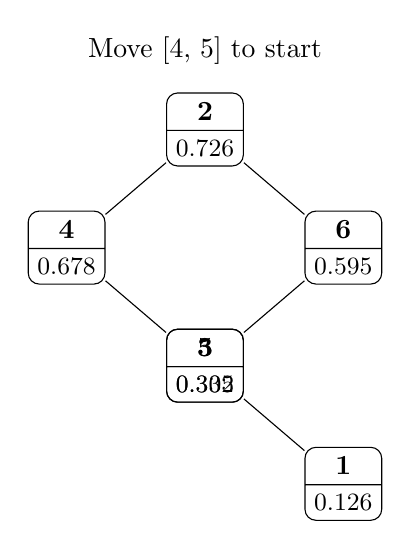
\begin{tikzpicture}[sibling distance=10em,every node/.style = {draw, align=center, shape=rectangle split,rectangle split parts=2, rounded corners}]
\node(root) { \textbf{2}\nodepart{second}{\small 0.726}} 
child { node { \textbf{4}\nodepart{second}{\small 0.678}} 
child[xshift=5em] { node { \textbf{5}\nodepart{second}{\small 0.302}} 
child[xshift=5em] { node { \textbf{1}\nodepart{second}{\small 0.126}}  } } }
child { node { \textbf{6}\nodepart{second}{\small 0.595}} 
child[xshift=-5em] { node { \textbf{3}\nodepart{second}{\small 0.335}}  } };
\node[shape=rectangle,draw=none,above of=root] {Move [4, 5] to start};
\end{tikzpicture}
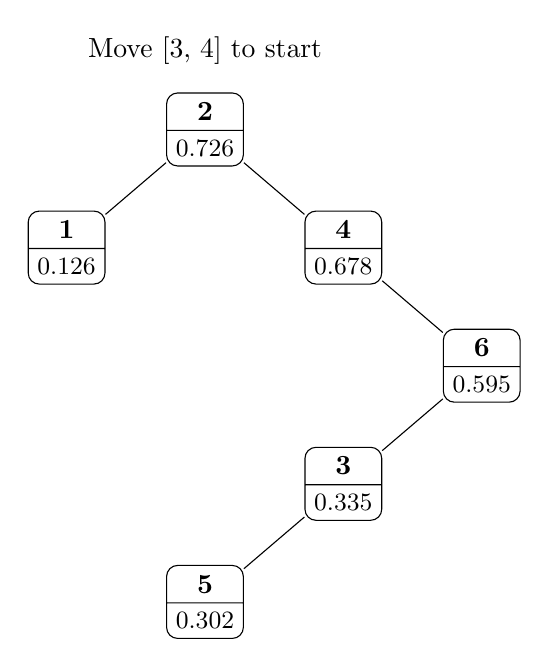
\begin{tikzpicture}[sibling distance=10em,every node/.style = {draw, align=center, shape=rectangle split,rectangle split parts=2, rounded corners}]
\node(root) { \textbf{2}\nodepart{second}{\small 0.726}} 
child { node { \textbf{1}\nodepart{second}{\small 0.126}}  }
child { node { \textbf{4}\nodepart{second}{\small 0.678}} 
child[xshift=5em] { node { \textbf{6}\nodepart{second}{\small 0.595}} 
child[xshift=-5em] { node { \textbf{3}\nodepart{second}{\small 0.335}} 
child[xshift=-5em] { node { \textbf{5}\nodepart{second}{\small 0.302}}  } } } };
\node[shape=rectangle,draw=none,above of=root] {Move [3, 4] to start};
\end{tikzpicture}
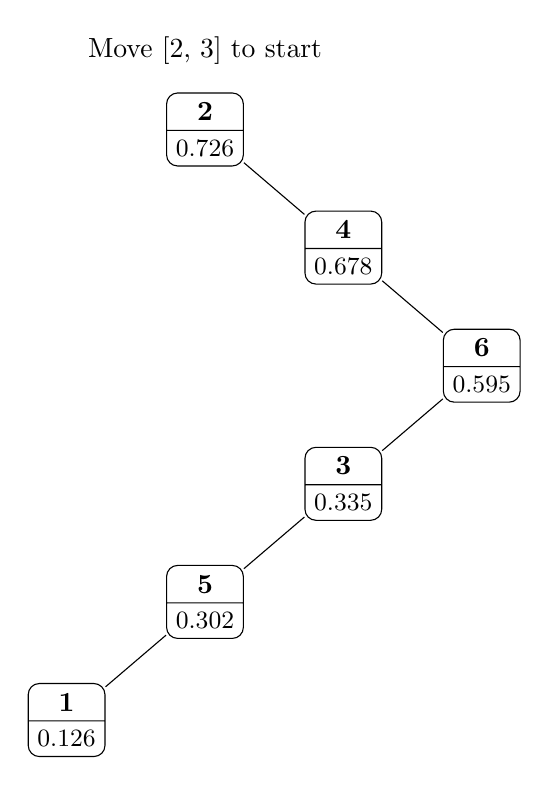
\begin{tikzpicture}[sibling distance=10em,every node/.style = {draw, align=center, shape=rectangle split,rectangle split parts=2, rounded corners}]
\node(root) { \textbf{2}\nodepart{second}{\small 0.726}} 
child[xshift=5em] { node { \textbf{4}\nodepart{second}{\small 0.678}} 
child[xshift=5em] { node { \textbf{6}\nodepart{second}{\small 0.595}} 
child[xshift=-5em] { node { \textbf{3}\nodepart{second}{\small 0.335}} 
child[xshift=-5em] { node { \textbf{5}\nodepart{second}{\small 0.302}} 
child[xshift=-5em] { node { \textbf{1}\nodepart{second}{\small 0.126}}  } } } } };
\node[shape=rectangle,draw=none,above of=root] {Move [2, 3] to start};
\end{tikzpicture}
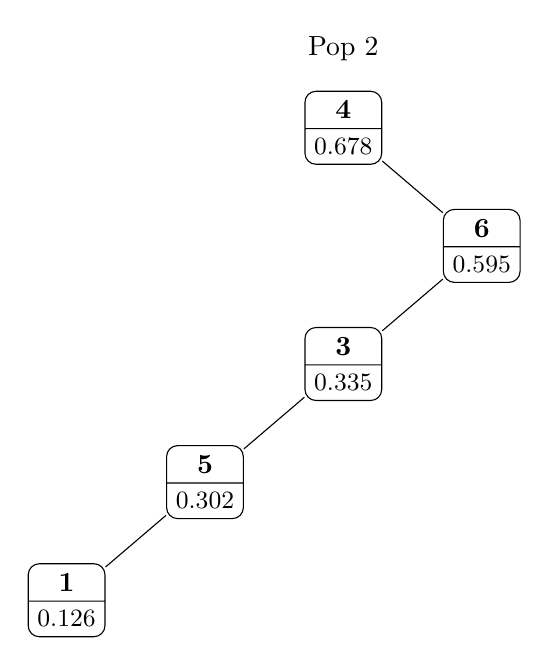
\begin{tikzpicture}[sibling distance=10em,every node/.style = {draw, align=center, shape=rectangle split,rectangle split parts=2, rounded corners}]
\node(root) { \textbf{4}\nodepart{second}{\small 0.678}} 
child[xshift=5em] { node { \textbf{6}\nodepart{second}{\small 0.595}} 
child[xshift=-5em] { node { \textbf{3}\nodepart{second}{\small 0.335}} 
child[xshift=-5em] { node { \textbf{5}\nodepart{second}{\small 0.302}} 
child[xshift=-5em] { node { \textbf{1}\nodepart{second}{\small 0.126}}  } } } };
\node[shape=rectangle,draw=none,above of=root] {Pop 2};
\end{tikzpicture}
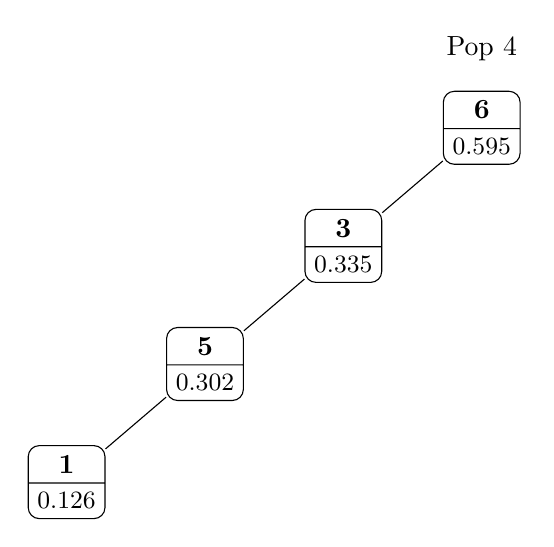
\begin{tikzpicture}[sibling distance=10em,every node/.style = {draw, align=center, shape=rectangle split,rectangle split parts=2, rounded corners}]
\node(root) { \textbf{6}\nodepart{second}{\small 0.595}} 
child[xshift=-5em] { node { \textbf{3}\nodepart{second}{\small 0.335}} 
child[xshift=-5em] { node { \textbf{5}\nodepart{second}{\small 0.302}} 
child[xshift=-5em] { node { \textbf{1}\nodepart{second}{\small 0.126}}  } } };
\node[shape=rectangle,draw=none,above of=root] {Pop 4};
\end{tikzpicture}
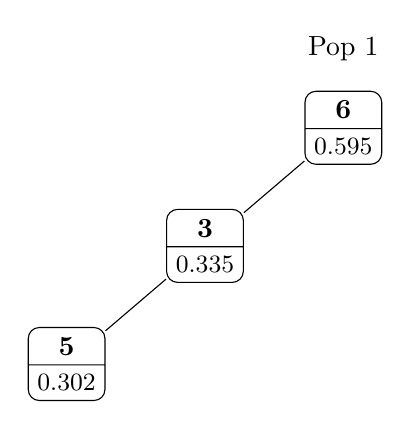
\begin{tikzpicture}[sibling distance=10em,every node/.style = {draw, align=center, shape=rectangle split,rectangle split parts=2, rounded corners}]
\node(root) { \textbf{6}\nodepart{second}{\small 0.595}} 
child[xshift=-5em] { node { \textbf{3}\nodepart{second}{\small 0.335}} 
child[xshift=-5em] { node { \textbf{5}\nodepart{second}{\small 0.302}}  } };
\node[shape=rectangle,draw=none,above of=root] {Pop 1};
\end{tikzpicture}
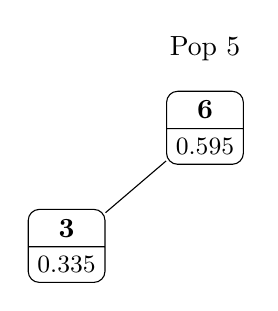
\begin{tikzpicture}[sibling distance=10em,every node/.style = {draw, align=center, shape=rectangle split,rectangle split parts=2, rounded corners}]
\node(root) { \textbf{6}\nodepart{second}{\small 0.595}} 
child[xshift=-5em] { node { \textbf{3}\nodepart{second}{\small 0.335}}  };
\node[shape=rectangle,draw=none,above of=root] {Pop 5};
\end{tikzpicture}
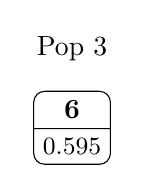
\begin{tikzpicture}[sibling distance=10em,every node/.style = {draw, align=center, shape=rectangle split,rectangle split parts=2, rounded corners}]
\node(root) { \textbf{6}\nodepart{second}{\small 0.595}} ;
\node[shape=rectangle,draw=none,above of=root] {Pop 3};
\end{tikzpicture}
\end{document}
